\documentclass[10pt]{article}
\usepackage[ngerman]{babel}
\usepackage[utf8]{inputenc}
\usepackage[T1]{fontenc}
\usepackage{amsmath}
\usepackage{amsfonts}
\usepackage{amssymb}
\usepackage[version=4]{mhchem}
\usepackage{stmaryrd}
\usepackage{bbold}
\usepackage{graphicx}
\usepackage[export]{adjustbox}
\graphicspath{ {./images/} }

\title{Hauptprüfung Abiturprüfung 2023 - Leistungsfach }

\author{Alexander Schwarz\\
www.mathe-aufgaben.com}
\date{}


\begin{document}
\maketitle
 Baden-Württemberg\section*{Pflichtteil - Aufgabensatz 2 \\
 Hilfsmittel: keine allgemeinbildende Gymnasien }


\section*{Aufgabe 1: (1 VP und 1,5 VP)}
Eine in $\mathbb{R}$ definierte ganzrationale, nicht lineare Funktion $f$ mit erster Ableitungsfunktion $\mathrm{f}^{\prime}$ und zweiter $\mathrm{f}^{\prime \prime}$ hat folgende Eigenschaften:

\begin{itemize}
  \item $f$ hat bei $x_{1}$ eine Nullstelle.
  \item Es gilt $f^{\prime}\left(x_{2}\right)=0$ und $f^{\prime \prime}\left(x_{2}\right) \neq 0$.
  \item $f^{\prime}$ hat ein Minimum an der Stelle $x_{3}$.
\end{itemize}

Die Abbildung in der Anlage zeigt die Position von $x_{1}, x_{2}$ und $x_{3}$.\\
a) Begründen Sie, dass der Grad von f mindestens 3 ist.\\
b) Skizzieren Sie in der Abbildung einen möglichen Graphen von $f$.

\section*{Aufgabe 2: (1 VP und 1,5 VP)}
Gegeben ist die in $\mathbb{R}$ definierte Funktion $f$ mit $\left.f(x)=-x^{2}+2 a x, a \in\right] 1 ;+\infty[$.\\
Die Nullstellen von f sind 0 und 2 a .\\
a) Zeigen Sie, dass das Flächenstück, das der Graph von f mit der x-Achse einschließt, den Inhalt $\frac{4}{3} a^{3}$ hat.\\
b) Der Hochpunkt des Graphen von fliegt auf einer Seite eines Quadrats; zwei Seiten dieses Quadrats liegen auf den Koordinatenachsen (vgl. Abbildung). Der Flächeninhalt des Quadrats stimmt mit dem Inhalt des Flächenstücks, das der Graph von f mit der x-Achse einschließt, überein. Bestimmen Sie den Wert von a.\\
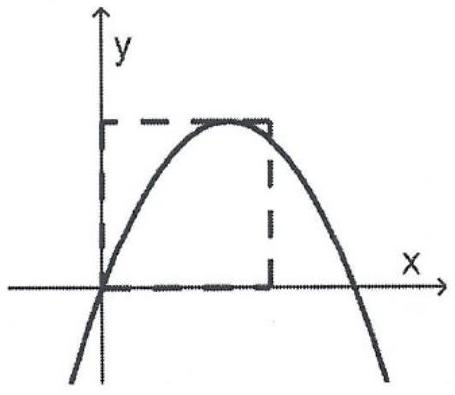
\includegraphics[max width=\textwidth, center]{2025_04_24_9b98536db296034492e8g-2}

\section*{Aufgabe 3: (1 VP und 1,5 VP)}
Abgebildet sind der Graph der Funktion $f$ mit $f(x)=\sin (\pi x)$ sowie eine Ursprungsgerade g mit der Steigung m.\\
a) Bestimmen Sie einen Term der Stammfunktion von f, deren Graph den Ursprung enthält.\\
b) Berechnen Sie den Wert von m, für den die Inhalte der beiden markierten Flächen gleich groß sind.\\
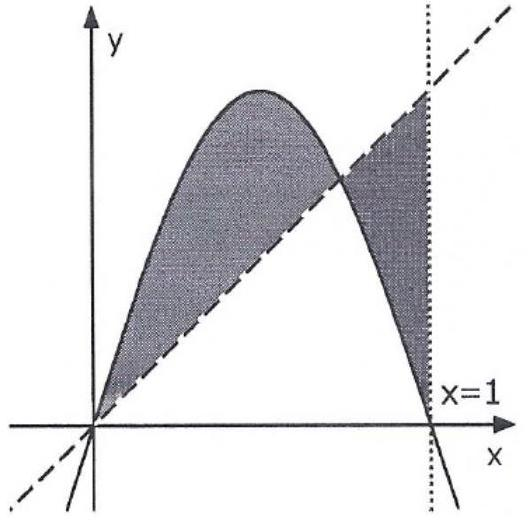
\includegraphics[max width=\textwidth, center]{2025_04_24_9b98536db296034492e8g-2(1)}

\section*{Aufgabe 4: (0,5 VP und 2 VP)}
Gegeben sind die Punkte $A(3|5| 5)$ und $B(1|1| 1)$ sowie die Geraden $g$ und $h$, die sich in B schneiden.\\
Die Gerade $g$ hat den Richtungsvektor $\left(\begin{array}{l}1 \\ 2 \\ 2\end{array}\right)$, die Gerade h den Richtungsvektor $\left(\begin{array}{l}1 \\ 0 \\ 0\end{array}\right)$.\\
a) Weisen Sie nach, dass $A$ auf $g$ liegt.\\
b) Bestimmen Sie die Koordinaten zweier Punkte $C$ und $D$ so, dass $C$ auf h liegt und das Viereck ABCD eine Raute ist.

\section*{Aufgabe 5: (1 VP und 1,5 VP)}
Ein Glücksrad besteht aus zwei Sektoren, die mit den Zahlen 2 bzw. 3 beschriftet sind. Die Wahrscheinlichkeit dafür, dass bei einmaligem Drehen die Zahl 2 erzielt wird, beträgt p. Bei einem Spiel dreht eine Person das Glücksrad genau so oft, bis die Summe der erzielten Zahlen 5, 6 oder 7 beträgt. Bei der Summe 6 gewinnt die Person das Spiel, sonst verliert sie.\\
a) Stellen Sie den Sachverhalt in einem beschrifteten Baumdiagramm dar.\\
b) Die beiden folgenden Ereignisse sind stochastisch unabhängig:

E: „Beim Drehen des Glücksrads wird die Zahl 2 erzielt."\\
G: „Die Person gewinnt das Spiel."\\
Ermitteln Sie eine Gleichung, die die Variable p enthält und die Berechnung des Werts von $p$ ermöglicht.

\section*{Aufgabe 6: (1 VP und 1,5 VP)}
In einen leeren Behälter werden drei Kugeln gelegt. Dabei wird die Farbe jeder Kugel durch Werfen eines Würfels festgelegt, dessen Seiten mit den Zahlen 1 bis 6 durchnummeriert sind: Wird die „1" oder die „2" erzielt, wird eine gelbe Kugel gewählt, sonst eine schwarze.\\
a) Weisen Sie rechnerisch nach, dass die Wahrscheinlichkeit dafür, dass sich nun mindestens zwei schwarze Kugeln im Behälter befinden, $\frac{20}{27}$ beträgt.\\
b) Aus dem Behälter werden zwei der drei Kugeln zufällig entnommen. Ermitteln Sie die Wahrscheinlichkeit dafür, dass beide entnommenen Kugeln schwarz sind.

\section*{Abbildung zu Aufgabe 1 (Pflichtteil Aufgabensatz 2)}
\begin{center}
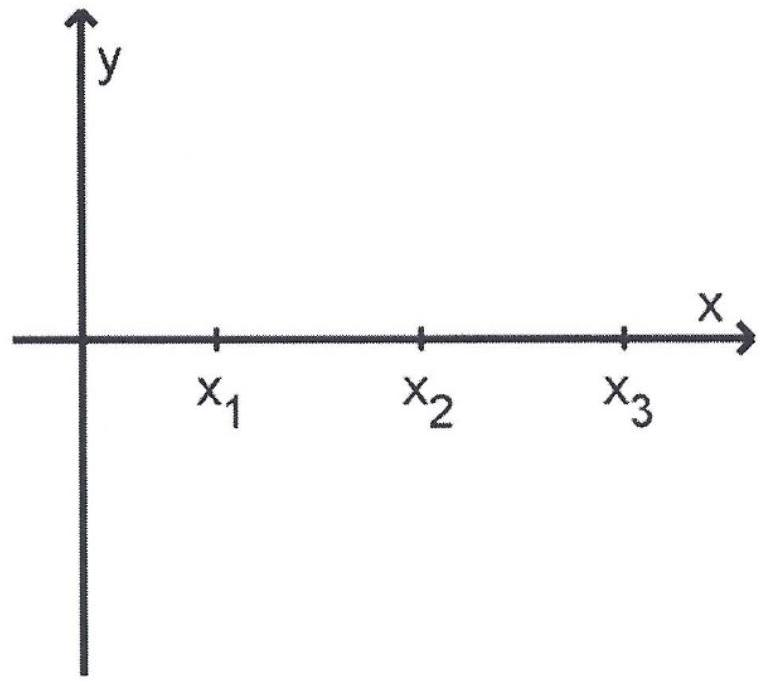
\includegraphics[max width=\textwidth]{2025_04_24_9b98536db296034492e8g-4}
\end{center}

\section*{Lösungen}
\section*{Aufgabe 1:}
a) Da $f^{\prime}$ an der Stelle $x_{3}$ ein Minimum hat, ist der Grad von $f^{\prime}$ mindestens 2.

Damit ist der Grad von $f$ mindestens 3.\\
b)

Der Graph von $f$ hat bei $x_{1}$ eine Nullstelle und bei $x_{2}$ eine Extremstelle und bei $x_{3}$ eine Wendestelle.\\
Da $f^{\prime}$ bei $x_{3}$ ein Minimum besitzt, besitzt die Wendestelle von f eine Tangente mit einer minimalen Steigung.\\
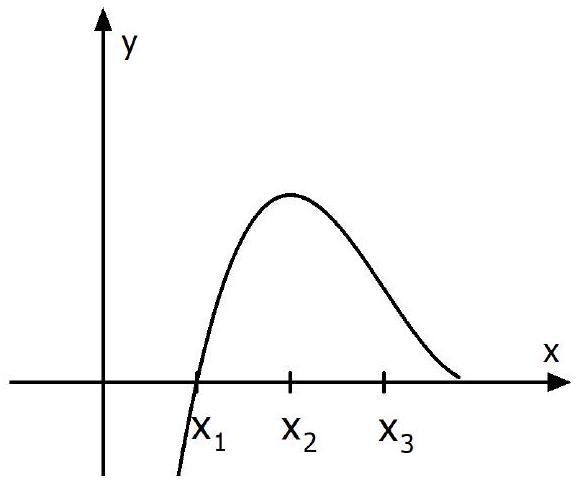
\includegraphics[max width=\textwidth, center]{2025_04_24_9b98536db296034492e8g-5}

\section*{Aufgabe 2:}
a) Berechnung des Flächeninhalts:

$$
A=\int_{0}^{2 a}\left(-x^{2}+2 a x\right) d x=\left[-\frac{1}{3} x^{3}+a x^{2}\right]_{0}^{2 a}=-\frac{8}{3} a^{3}+4 a^{3}-0=\frac{4}{3} a^{3}
$$

b) Da die Nullstellen von $f$ bei $x=0$ und $x=2 a$ sind, besitzt der Hochpunkt aus Symmetriegründen die Koordinaten $\mathrm{H}(\mathrm{a} \mid \mathrm{f}(\mathrm{a})$ ).\\
Es gilt $f(a)=-a^{2}+2 a^{2}=a^{2}$, das heißt die Breite des Quadrats (und damit auch die Länge des Quadrats) ist $a^{2}$.\\
Flächeninhalt des Quadrats: $A_{Q}=a^{2} \cdot a^{2}=a^{4}$\\
Bedingung: $a^{4}=\frac{4}{3} a^{3} \Leftrightarrow a^{4}-\frac{4}{3} a^{3}=0 \Leftrightarrow a^{3} \cdot\left(a-\frac{4}{3}\right)=0$\\
Lösung mit dem Satz vom Nullprodukt: a = 0 (scheidet als Lösung aus, da laut Aufgabenstellung $\mathrm{a}>1$ sein soll) und $\mathrm{a}=\frac{4}{3}$.\\
Somit gilt $\mathrm{a}=\frac{4}{3}$.

\section*{Aufgabe 3:}
a) Stammfunktion von $f(x)=\sin (\pi x)$ :

$$
F(x)=-\frac{1}{\pi} \cos (\pi x)+C
$$

Bedingung: $F(0)=0 \Rightarrow-\frac{1}{\pi}+C=0 \Rightarrow C=\frac{1}{\pi}$\\
Die gesuchte Stammfunktion lautet $F(x)=-\frac{1}{\pi} \cos (\pi x)+\frac{1}{\pi}$\\
b) Die Gerade $g$ hat die Gleichung $y=m x$.

Die beiden Flächenstücke werden jeweils vom Schaubild von f und der Geraden g oben und unten einschlossen.

Linkes Flächenstück: $A_{\text {links }}=\int_{0}^{\text {Schnitstelle }}(f(x)-m x) d x$\\
Rechtes Flächenstück: $A_{\text {rechts }}=\int_{\text {Schnitstelle }}^{1}(m x-f(x)) d x$\\
Bedingung: $A_{\text {links }}-A_{\text {rechts }}=0 \Leftrightarrow A_{\text {links }}+\left(-A_{\text {rechts }}\right)=0$\\
$\Leftrightarrow \int_{0}^{\text {Schnitstelle }}(f(x)-m x) d x+\left(-\int_{\text {Schnitstelle }}^{1}(m x-f(x)) d x\right)=0$\\
$\Leftrightarrow \int_{0}^{\text {Schnitstelle }}(f(x)-m x) d x+\int_{\text {Schnitstelle }}^{1}(f(x)-m x) d x=0$\\
$\Leftrightarrow \int_{0}^{1}(f(x)-m x) d x=0$\\
$\int_{0}^{1}(f(x)-m x) d x=\left[-\frac{1}{\pi} \cos (\pi x)-\frac{1}{2} m x^{2}\right]_{0}^{1}=-\frac{1}{\pi} \cdot(-1)-\frac{1}{2} m-\left(-\frac{1}{\pi}\right)=\frac{2}{\pi}-\frac{1}{2} m$\\
$\frac{2}{\pi}-\frac{1}{2} m=0 \Leftrightarrow m=\frac{4}{\pi}$

\section*{Aufgabe 4:}
a) Gleichung der Geraden $\mathrm{g}: \overrightarrow{\mathrm{x}}=\left(\begin{array}{l}1 \\ 1 \\ 1\end{array}\right)+\mathrm{r} \cdot\left(\begin{array}{l}1 \\ 2 \\ 2\end{array}\right)$

Prüfung, ob $A(3|5| 5)$ auf g liegt: $\left(\begin{array}{l}3 \\ 5 \\ 5\end{array}\right)=\left(\begin{array}{l}1 \\ 1 \\ 1\end{array}\right)+r \cdot\left(\begin{array}{l}1 \\ 2 \\ 2\end{array}\right) \quad \begin{aligned} 3 & =1+r \\ 5 & =1+2 r \\ 5 & =1+2 r\end{aligned}$\\
Das LGS wird für $r=2$ erfüllt, also liegt A auf g .\\
b) Skizze:\\
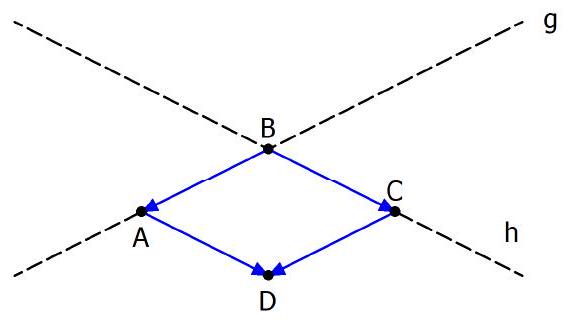
\includegraphics[max width=\textwidth, center]{2025_04_24_9b98536db296034492e8g-7}

Länge der Strecke $\overline{\mathrm{AB}}: \left.|\overrightarrow{\mathrm{AB}}|=\left(\begin{array}{l}-2 \\ -4 \\ -4\end{array}\right) \right\rvert\,=6$\\
1.Lösungsmöglichkeit:

Koordinaten von $\mathrm{C}: \overrightarrow{\mathrm{OC}}=\overrightarrow{\mathrm{OB}}+6 \cdot\left(\begin{array}{l}1 \\ 0 \\ 0\end{array}\right)=\left(\begin{array}{l}1 \\ 1 \\ 1\end{array}\right)+\left(\begin{array}{l}6 \\ 0 \\ 0\end{array}\right)=\left(\begin{array}{l}7 \\ 1 \\ 1\end{array}\right)$, also $\mathrm{C}(7|1| 1)$\\
Koordinaten von $\mathrm{D}: \overrightarrow{\mathrm{OD}}=\overrightarrow{\mathrm{OA}}+\overrightarrow{\mathrm{BC}}=\left(\begin{array}{l}3 \\ 5 \\ 5\end{array}\right)+\left(\begin{array}{l}6 \\ 0 \\ 0\end{array}\right)=\left(\begin{array}{l}9 \\ 5 \\ 5\end{array}\right)$, also $\mathrm{D}(9|5| 5)$\\
2.Lösungsmöglichkeit:

Koordinaten von $\mathrm{C}: \overrightarrow{\mathrm{OC}}=\overrightarrow{\mathrm{OB}}-6 \cdot\left(\begin{array}{l}1 \\ 0 \\ 0\end{array}\right)=\left(\begin{array}{l}1 \\ 1 \\ 1\end{array}\right)-\left(\begin{array}{l}6 \\ 0 \\ 0\end{array}\right)=\left(\begin{array}{c}-5 \\ 1 \\ 1\end{array}\right)$, also $\mathrm{C}(-5|1| 1)$\\
Koordinaten von $\mathrm{D}: \overrightarrow{\mathrm{OD}}=\overrightarrow{\mathrm{OA}}+\overrightarrow{\mathrm{BC}}=\left(\begin{array}{l}3 \\ 5 \\ 5\end{array}\right)+\left(\begin{array}{c}-6 \\ 0 \\ 0\end{array}\right)=\left(\begin{array}{c}-3 \\ 5 \\ 5\end{array}\right)$, also $\mathrm{D}(-3|5| 5)$

\section*{Aufgabe 5:}
a) Baumdiagramm:\\
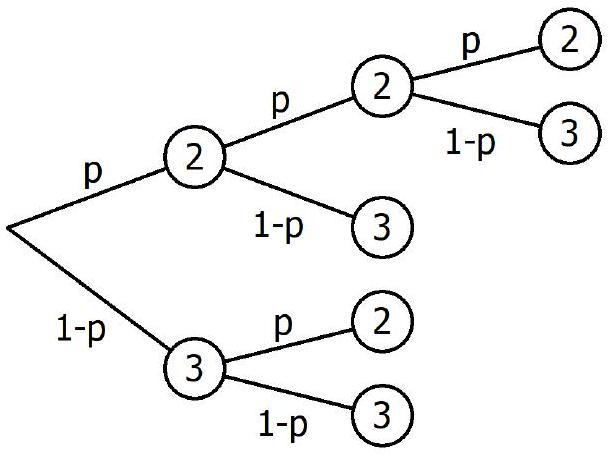
\includegraphics[max width=\textwidth, center]{2025_04_24_9b98536db296034492e8g-7(1)}\\
b) Bedingung für die Unabhängigkeit der Ereignisse $E$ und $G: P(E \cap G)=P(E) \cdot P(G)$

$$
\begin{aligned}
& P(G)=P(222)+P(33)=p^{3}+(1-p)^{2} \\
& P(E)=p \\
& P(E \cap G)=P(222)=p^{3} \\
& \Rightarrow p^{3}=p \cdot\left[p^{3}+(1-p)^{2}\right] \quad \mid: p \\
& \Leftrightarrow p^{2}=p^{3}+(1-p)^{2}
\end{aligned}
$$

\section*{Aufgabe 6:}
a) $\mathrm{P}($ mindestens zwei schwarze Kugeln $)=\mathrm{P}(2$ schwarze $)+\mathrm{P}(3$ schwarze $)$\\
$\frac{2}{3} \cdot \frac{2}{3} \cdot \frac{1}{3} \cdot 3+\left(\frac{2}{3}\right)^{3}=\frac{12}{27}+\frac{8}{27}=\frac{20}{27}$ was zu zeigen war\\
Hinweis: Der Faktor 3 ergibt sich aufgrund der Möglichkeiten ssg, sgs, gss.\\
b) Es können nur dann zwei schwarze Kugeln entnommen werden, wenn sich in der Urne mindestens 2 schwarze Kugeln befinden.\\
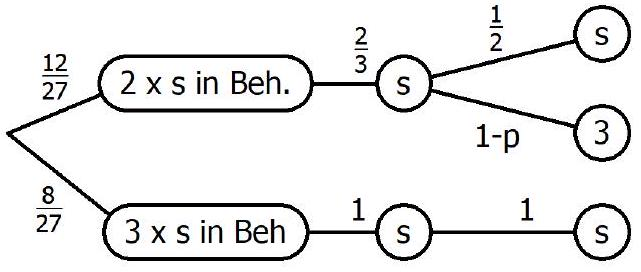
\includegraphics[max width=\textwidth, center]{2025_04_24_9b98536db296034492e8g-8}\\
$P(2$ schwarze Kugeln werden gezogen $)=\frac{12}{27} \cdot \frac{2}{3} \cdot \frac{1}{2}+\frac{8}{27} \cdot 1 \cdot 1=\frac{4}{27}+\frac{8}{27}=\frac{12}{27}$


\end{document}